\documentclass[runningheads]{llncs}
\usepackage{graphicx}
\usepackage{booktabs}
\usepackage{amsmath}
\usepackage{url}

\begin{document}

\title{Trustworthy AI for Cervical Cytology Screening Does Not Compose: Independent Verification of Efficiency, Domain-Shift Robustness, Uncertainty Quantification, and Explainability}
\titlerunning{Trustworthy AI for Cervical Cytology Screening Does Not Compose}

\author{Anonymous Author(s)}
\authorrunning{Anonymous Author(s)}
\institute{Submitted for double-blind review}

\maketitle

\begin{abstract}
``Trustworthy AI'' is usually evaluated as if it were one property a
pipeline either has or lacks. We show instead that, for a cervical
cytology screening pipeline, it decomposes into at least five
independently-varying claims -- whether the most parameter-efficient
model is also the safest to deploy, whether any static model property
predicts domain-shift robustness, whether an uncertainty-quantification
method's own native confidence signal correctly flags that a model has
entered a failure regime, whether combining two such signals helps, and
which explainability method is most faithful -- and that testing all five
side by side on one fixed pipeline, rather than picking one and assuming
the others follow the same pattern, is itself this paper's central
contribution. First, benchmarking 12 models spanning CNN, full-size vision
transformer, and efficient-vision-transformer families on SIPaKMeD
cervical cytology classification, then evaluating the same models
zero-shot on three independent external shift datasets (Herlev, Mendeley
LBC, APCEM), we find that the two most parameter-efficient models in the
registry ($\sim$2.1M parameters each) are also the two most accurate in
distribution -- efficiency costs nothing here -- yet the overall
in-distribution winner (EfficientViT-M0) is the worst-performing model of
all 12 on two of the three external datasets, dropping below the chance
floor on one; no static property we measured (parameter count, FLOPs,
in-distribution accuracy, architecture family) reliably predicts which
model fails safely, and a CNN-family robustness pattern that survives two
independent shift datasets collapses on the third. A full-registry
seed-variance check (all 12 models retrained at 2 further seeds) shows
this instability runs deeper than model identity: the same model can move
from in-distribution winner to mid-pack shift performer under nothing
more than a different random seed, so even this paper's own illustrative
example should be read as one-seed evidence for a stable higher-level
claim, not a reproducible model-level fact. Second, comparing four
uncertainty-quantification methods' own cheapest native confidence
signals on this exact backbone, method ranking itself inverts with shift
severity in our original run: a five-member deep ensemble wins clearly
under moderate shift, while MC Dropout's entropy is the only signal that
substantially improves failure detection under severe shift -- but a
paired-bootstrap significance test, followed by three independent
retrainings of MC Dropout under an identical recipe, shows this specific
severe-shift ranking does not reproduce (Mendeley LBC risk-coverage AUC
spans 0.285--0.503 across four otherwise-identical training runs, a wider
spread than separates any two \emph{different} methods), and no method
reaches a reliable abstention operating point under severe shift in
either run. Third, testing explainability method choice, uncertainty-
signal composition, and measured deployment cost side by side on the same
pipeline: relevancy propagation wins cleanly against attention rollout and
Grad-CAM on both behavioral faithfulness and real expert-annotated nucleus
localization, with no condition-dependent flip, and this ranking
replicates exactly on a second, independently-trained backbone;
combining two uncertainty signals for selective prediction helps only
under the one condition where the better individual signal was already
failing, and hurts where that signal was already excellent; and
resource-efficiency claims evaluated by parameter count and FLOPs alone do
not reliably predict real CPU latency, while returning an explanation
alongside a prediction costs roughly 3.3$\times$ a bare forward pass.
Across five tested properties, three distinct resolution patterns emerge
-- clean and condition-independent (explainability method choice),
conditional on the operating regime (uncertainty method choice, signal
composition, and which specific model illustrates a given claim), and
existing only once directly measured (deployment cost, architecture-
family robustness patterns) -- meaning a trustworthy medical AI pipeline
cannot be verified with one strategy applied uniformly to every
component; each property needs its own test, on its own terms, and a
single seed, backbone, or shift dataset is not enough to certify any of
them.

\keywords{Cervical cytology \and Vision transformers \and Domain shift \and Model efficiency \and Uncertainty quantification \and Calibration \and Selective prediction \and Conformal prediction \and Explainable AI \and Trustworthy medical AI}
\end{abstract}

\section{Introduction}

Cervical cancer remains substantially more curable when caught at a
localized stage, yet screening access is documented to be uneven across
rural and urban U.S.\ counties, and a growing literature proposes vision
transformers -- often marketed as ``efficient'' or ``lightweight''
variants -- as classification backbones for automated cytology screening
in specialist-scarce settings. A screening tool that fails silently --
misclassifying confidently under conditions its training data did not
cover -- is more dangerous than one that fails and flags the failure, so
deploying such a tool responsibly requires more than one property to hold:
the backbone must be accurate \emph{and} robust to the distribution shift
it will inevitably meet across institutions, scanners, and populations;
if it fails anyway, some confidence signal must correctly flag that
failure; and if a clinician is to act on its output, its explanation must
be faithful, not merely plausible-looking. ``Trustworthy AI'' is usually
evaluated as if it were one property a pipeline either has or lacks. This
paper's central argument is that it is not: we identify five
independently-varying claims underlying a trustworthy cervical cytology
screening pipeline and test each one directly, on one fixed pipeline,
rather than assuming that verifying one property licenses assuming the
others.

The five claims, and how each is tested, are: (1) does a lightweight,
parameter-efficient architecture trade accuracy for efficiency, tested
across a 12-model registry in distribution; (2) does whichever backbone
wins that in-distribution benchmark remain the safest choice under real
cross-institution domain shift, tested zero-shot on three independent
external datasets and, because a single seed cannot answer a question
about reproducibility, re-tested across three random seeds per model;
(3) does a standard uncertainty-quantification method's own native
confidence signal correctly detect that a backbone has entered a shift
regime where its predictions should not be trusted, tested across four
methods and two shift severities, and, because a single training run
cannot answer a question about a method's stability, re-tested via a
significance test and repeated retraining; (4) does combining two
uncertainty signals into one selective-prediction rule help, tested
directly rather than assumed from either signal's individual behavior;
and (5) which explainability method is most faithful, tested against both
behavioral faithfulness and real expert-annotated ground truth, and
re-tested on a second, independently-trained backbone. A sixth,
supporting thread runs throughout: whether architectural efficiency claims
and OOD-confidence-drop claims hold under direct measurement rather than
assumption, which turns out to require its own verification as much as
any of the five main claims.

Our contributions are organized around these five properties, plus two
cross-cutting methodological points that only emerge from testing them
side by side rather than in isolation. First, a 12-model efficiency/accuracy
benchmark on cervical cytology classification showing that the most
parameter-efficient models in the registry are also the most accurate --
efficiency costs nothing here, contrary to the usual trade-off framing.
Second, a systematic escalation from a 2-model to a 4-model to a full
12-model cross-dataset domain-shift evaluation across three independent
external datasets, converging on: no single static model property
predicts shift robustness, the in-distribution winner is the
shift-robustness loser, and a robustness pattern that survives two shift
datasets is not guaranteed to survive a third. Third, a full-registry
seed-variance check across all 12 models at 3 random seeds each, showing
that some of the paper's own illustrative single-model, single-dataset
claims -- including its own headline poster-child example -- are
seed-specific rather than general, a finding that reinforces rather than
undermines the paper's central thesis by extending ``no static property
predicts robustness'' from across models to across seeds of the same
model. Fourth, a four-method uncertainty-quantification comparison on the
backbone identified in contribution 2 as having a documented, severe, real
distribution-shift failure, showing that method ranking itself depends on
shift severity -- and a significance test plus three independent
retrainings showing that even the specific severe-shift ranking reported
here does not reliably reproduce, a second, sharper layer of the same
warning contribution 3 raises about individual models. Fifth, the first
system-level test of whether combining two uncertainty signals for
selective prediction helps, finding a conditional answer that extends
``no single best method'' from individual methods to method combinations.
Sixth, a three-way explainability comparison against both behavioral
faithfulness and real expert-annotated localization ground truth, where
one method wins unambiguously on every metric and replicates exactly on a
second backbone -- a cleaner, more stable result than any of the
uncertainty-related findings, and evidence that not every property of a
trustworthy pipeline is equally fragile. Seventh, a measured, not
estimated, resource-efficiency and deployment-cost analysis showing that
parameter count and FLOPs do not reliably predict CPU latency, and that an
explanation costs $\sim$3.3$\times$ a bare forward pass. The pattern
across all seven -- some claims collapse under retraining, some flip with
operating condition, and some hold cleanly but only once actually
measured -- is the paper's unifying argument: a trustworthy-AI pipeline
cannot be verified with one strategy applied uniformly across its
components, and each property needs its own, independent, and where
possible repeated test.

\section{Related Work}

\subsection{Efficient vision transformers}

Efficiency-oriented vision transformer variants form three loose lineages
relevant to the registry benchmarked here. Hybrid local--global designs
(MobileViT \cite{mehta2022mobilevit}, MobileViTv2
\cite{mehta2022mobilevitv2}) interleave convolutional stages with
transformer blocks to keep early-stage compute cheap while retaining
global attention at coarser resolutions. Distillation-oriented designs
(DeiT \cite{touvron2021deit}) instead keep a standard ViT backbone but use
a distillation token and teacher network to reach competitive accuracy at
far smaller pretraining-data budgets than the original ViT
\cite{dosovitskiy2021vit} required. Hardware-aware designs (LeViT
\cite{graham2021levit}, TinyViT \cite{wu2022tinyvit}) reintroduce
convolutional stages specifically to improve real-device latency, not
just FLOP count, by favoring operations that map efficiently onto
standard inference kernels. EfficientViT-M0 and EfficientViT-B0, the two
smallest and most accurate models in this study, are frequently assumed to
share a lineage because timm's tag naming groups them together --
verified directly rather than assumed, they do not. EfficientViT-M0 uses
cascaded group attention \cite{liu2023efficientvit}, a Microsoft-authored
design that reduces redundant computation across attention heads by
feeding each head a different split of the input feature map.
EfficientViT-B0 belongs to an entirely unrelated MIT-authored lineage
built around multi-scale linear attention for high-resolution dense
prediction \cite{cai2023efficientvit}, originally designed for
segmentation and detection rather than classification efficiency. That
this study's two best-performing, most-efficient models come from two
architecturally unrelated papers sharing only a name is itself a small
caution against treating ``the EfficientViT family'' as one coherent
design lineage in future efficiency claims. None of these efficiency-
oriented design papers evaluate cross-institution domain shift as part of
their own efficiency claim -- efficiency and robustness are treated as
separate, unrelated properties in the architecture literature this
registry draws from, which is precisely the gap Sections~4.1--4.4 address.

\subsection{Domain shift and model selection in medical imaging}

A substantial general (not cervical-cytology-specific) medical-imaging
literature documents that models selected on held-out in-distribution
data can degrade sharply under real-world distribution shift across
scanners, sites, and populations, motivating external-validation
practices increasingly required by regulators and journals alike.
However, this literature typically evaluates one or a small number of
architectures rather than a systematic sweep across CNN, full-size
transformer, and efficient-transformer families at matched task and data
scale, which is what distinguishes this paper's 12-model, three-shift-
dataset design: the question is not whether shift degrades performance
(well established) but \emph{whether any measurable static property of a
model predicts which model degrades least}, tested directly rather than
assumed from a single architecture's behavior.

\subsection{Post-hoc calibration and its limits under shift}

Temperature scaling \cite{guo2017calibration} remains the standard
post-hoc softmax calibration baseline: a single scalar fit on a held-out
split rescales logits so that in-distribution confidence matches
empirical accuracy, at essentially zero added inference cost. It is a
strong in-distribution baseline (Section~4.5) but is a purely
in-distribution correction by construction -- it cannot introduce
information the model did not already encode about out-of-distribution
inputs, which is exactly why it is the weakest signal once shift severity
increases (Section~4.5). This motivates comparing it against methods that
inject additional signal at training or inference time rather than only
recalibrating a fixed model's existing outputs.

\subsection{Multi-pass and ensemble uncertainty}

MC Dropout \cite{gal2016dropout} approximates Bayesian inference by
keeping dropout active at test time and treating the spread across
repeated stochastic forward passes as an uncertainty signal, at a cost
proportional to the number of passes. Deep ensembles
\cite{lakshminarayanan2017ensembles} instead train several independently-
initialized models and use their disagreement, at a cost proportional to
ensemble size; empirically, ensemble diversity has been argued in the
broader literature to capture a different, complementary source of
uncertainty (functional diversity across independently-trained models)
than a single model's own stochastic-forward-pass variance, which is
consistent with this paper's finding (Section~4.5) that the two methods
are not redundant with each other -- they win under different shift
severities rather than one strictly dominating the other.

\subsection{Single-pass uncertainty and evidential learning}

Evidential deep learning \cite{sensoy2018evidential} reframes
classification as Dirichlet evidence accumulation, producing a
single-pass uncertainty signal (vacuity) without the multi-pass or
multi-model inference cost MC Dropout and deep ensembles incur -- an
attractive property for latency-constrained deployment, and the reason it
is included here despite calibrating markedly worse than the other three
methods in distribution (Section~4.5). Whether that single-pass efficiency
advantage is worth its calibration cost is precisely an empirical,
task-dependent question this comparison is designed to answer rather than
assume from the method's design motivation alone.

\subsection{Uncertainty quantification in cervical cancer screening}

Adjacent work applies conformal prediction and Monte Carlo inference
specifically to cervical cancer screening uncertainty, typically
proposing or evaluating one uncertainty method in isolation against a
single baseline. This paper differs by comparing four methods head-to-head
on a documented real (not assumed or synthetically induced) shift-failure
case, by evaluating each method across two shift severities rather than
one -- which is precisely what reveals the rank inversion in Section~4.5
a single-severity evaluation could not have surfaced -- and, further, by
testing whether that inversion itself survives retraining
(Section~4.6), a question adjacent single-run comparisons in this
literature do not typically ask of themselves.

\subsection{Transformer explainability methods}

Attention rollout \cite{abnar2020quantifying} treats a transformer's own
attention weights, chained across layers via a fixed recurrence, as a
relevance signal, on the premise that attention indicates where a model
``looks.'' This premise has itself been contested in the broader
literature examining whether attention weights are faithful explanations
of a model's actual decision process rather than merely correlated with
it -- a concern this paper's own faithfulness metrics (Section~4.7) are
designed to test empirically rather than assume either way. Relevancy
propagation \cite{chefer2021transformer} extends attention rollout by
weighting each transformer block's attention matrix with its gradient
with respect to the target class before the same rollout aggregation,
making the resulting relevance map class-discriminative rather than a
fixed structural property of attention, and is the primary method
evaluated here specifically because it addresses the class-agnosticity
critique of raw attention directly. Grad-CAM \cite{selvaraju2017gradcam}
was originally designed for CNN feature maps, where a single late
convolutional layer naturally encodes class-relevant spatial structure;
its adaptation to transformers by targeting a block's token-wise
activations instead of a convolutional feature map is common practice in
the literature, but the specific failure mode we identify and document
(Section~3.6) for CLS-token-pooled ViTs -- an all-zero heatmap if the
wrong block is targeted -- does not appear to be widely flagged in prior
adaptations, despite being silent rather than an error.

\subsection{Selective prediction and conformal calibration}

Split conformal prediction provides a distribution-free, finite-sample
coverage guarantee from a single calibration split, at the cost of
producing a set of plausible labels rather than one score; its prediction
set size is a natural, model-agnostic uncertainty proxy, but one that is
coarse (a small integer count) compared to a continuous confidence score.
This paper's system-integration question -- whether combining
temperature-scaled confidence with conformal set size outperforms either
alone (Section~4.9) -- is, to our knowledge, not directly addressed by
prior work proposing either signal independently, since each is typically
evaluated as a self-contained method rather than as one input to a
combined abstention rule.

\subsection{Faithfulness evaluation}

Deletion/insertion faithfulness \cite{petsiuk2018rise} evaluates an
explanation by its behavioral effect on the model itself (does removing
or revealing the patches an explanation calls important actually change
the model's prediction), rather than by agreement with a human-annotated
region, and is the behavioral-faithfulness metric used throughout
Section~4.7. Evaluating localization against SIPaKMeD's own expert-marked
nucleus polygons, rather than a segmentation model's derived output,
avoids compounding this paper's explainability evaluation with a second
model's own errors.

\subsection{Closely related prior work}

Directly adjacent to this paper's own scope: a stacking-ensemble approach
combined with explainable AI for cervical cancer diagnosis
\cite{mohiuddin2025}, which this paper differs from by evaluating
explainability methods against a real expert-annotated localization
ground truth and behavioral faithfulness metrics, and by evaluating
efficiency--robustness trade-offs across a full 12-model architecture-
family registry, rather than an ensemble-accuracy framing over a single
model; and a lightweight-ViT-plus-explainability design for plant disease
diagnosis, ``MaizeFormerX'' \cite{rahman2026maizeformerx}, which
motivates this paper's own choice to hold efficiency and explainability as
joint, not competing, design goals. Two further papers sit in adjacent
clinical-AI territory: a semi-supervised retinal disease recognition
system \cite{gony2026retinal} and an explainable multimodal AI framework
with reinforcement learning for post-surgical clinical decision support
\cite{ahmed2026postsurgical}, both part of a broader body of work in
trustworthy, explainable clinical AI of which this paper's cervical
cytology pipeline is one instance.

\section{Methods}

\subsection{Overview: which backbone answers which question}

Three of this paper's five properties (efficiency, shift robustness, and
its seed-variance check) are tested across the full 12-model registry
(Section~3.3), since the question there is precisely whether backbone
identity predicts an outcome, which requires varying backbone identity.
The uncertainty-quantification comparison (Section~3.5) instead holds one
backbone fixed -- EfficientViT-M0, the registry's in-distribution winner
and, per Section~4.2, its worst-performing model under two of three
external shifts -- to isolate the uncertainty-quantification method
rather than architecture, and because this is the exact backbone for
which the question ``can a confidence signal flag this specific failure''
is most practically urgent. The explainability comparison (Section~3.6)
uses a third backbone, DeiT-Tiny, instead: relevancy propagation and
attention rollout are both defined only for standard multi-head
self-attention transformer blocks, and EfficientViT-M0's hybrid
convolutional + cascaded-group-attention design has no established
propagation rule for either method, so forcing an ad hoc extension onto
an architecture these methods were not designed for was avoided in favor
of a standard \texttt{timm} \texttt{VisionTransformer} (DeiT-Tiny, 0.9606
balanced accuracy on the same in-distribution task, vs.\ EfficientViT-M0's
0.9654) retrained fresh for this purpose. The explainability ranking is
re-tested on a second, independently-trained backbone of the same family
(ViT-Small, Section~4.8) to confirm it is not one lucky model's property;
the system-integration and resource-efficiency results (Sections~4.9--4.10)
reuse DeiT-Tiny and the Herlev/Mendeley LBC shift conditions established
in Section~3.4.

\subsection{Datasets}

\textbf{SIPaKMeD} \cite{plissiti2018sipakmed} (4,049 native-resolution
single-cell crops derived directly from the dataset's own
cytoplasm-polygon boundary annotations, not a pre-resized third-party
mirror) is the in-distribution training and test dataset throughout, with
5 Bethesda-relevant cytomorphology classes. Three independent external
datasets provide zero-shot cross-institution shift evaluation, harmonized
onto one shared binary normal/abnormal label: \textbf{Herlev}
\cite{jantzen2005herlev} (moderate shift), \textbf{Mendeley LBC}
\cite{hussain2020mendeley} (severe shift), and the
\textbf{APCEM-Enhanced Cervical Cytology Pap Smear Image Dataset}
\cite{aswini2026apcem} (4,253 images across the 6-class Bethesda taxonomy
-- NILM, ASC-US, ASC-H, LSIL, HSIL, SSC -- harmonized identically: NILM
normal, all five atypical/dysplastic classes abnormal). APCEM differs from
Herlev and Mendeley LBC in acquisition pipeline, institution, and label
granularity, so it functions as a genuinely independent replication of
the domain-shift evaluation rather than a second look at the same shift.

\subsection{Model registry}

Twelve models spanning three families: CNN baselines (ResNet-50
\cite{he2016resnet}, MobileNetV2 \cite{sandler2018mobilenetv2},
EfficientNet-Lite0 \cite{tan2019efficientnet}), full-size vision
transformers (ViT-Small \cite{dosovitskiy2021vit}, Swin-Tiny
\cite{liu2021swin}), and efficient/mobile-oriented vision transformers
(DeiT-Tiny \cite{touvron2021deit}, LeViT-128 \cite{graham2021levit},
TinyViT-5M \cite{wu2022tinyvit}, MobileViT-S \cite{mehta2022mobilevit},
MobileViTv2 \cite{mehta2022mobilevitv2}, EfficientViT-B0
\cite{cai2023efficientvit}, EfficientViT-M0 \cite{liu2023efficientvit}).
All timm tags verified against the pinned timm version rather than assumed
from memory; the two EfficientViT variants' source papers were confirmed
independently against timm's own model cards rather than assumed from the
shared tag prefix (Section~2.1).

\subsection{Training and in-distribution evaluation}

All 12 models trained on SIPaKMeD, 60/15/10/15
train/val/calibration/test split, seed 13 as the headline seed (extended
to seeds 17 and 29 for the seed-variance check, Section~4.4), full
30-epoch budget with early stopping (patience 7), on a single GPU.
Reported: balanced accuracy, macro F1, AUROC, parameter count, and
measured (not estimated) inference latency.

\subsection{Cross-dataset domain-shift evaluation}

Each model evaluated zero-shot -- no retraining, no recalibration -- on
Herlev, Mendeley LBC, and APCEM after harmonizing all datasets' differing
label taxonomies onto one shared binary normal/abnormal label. This tests
generalization under the conditions this application will actually face:
different institutions, scanners, and staining protocols, not a synthetic
corruption of the same source images. The seed-variance check
(Section~4.4) repeats this protocol for all 12 models at 2 further seeds,
training once per model per seed and evaluating the same checkpoint on
all three external datasets, rather than retraining separately per
dataset.

\subsection{Uncertainty-quantification methods}

Four methods, each using its own cheapest native confidence signal (a
single native signal, not a method-specific post-hoc correction layered
on top, so the comparison reflects what a deployed system would actually
have access to without extra engineering), all sharing one manifest, one
calibration split, and one backbone initialization recipe (EfficientViT-M0):
(1) \textbf{Baseline}: cross-entropy training, post-hoc temperature
scaling fit on a held-out calibration split; confidence = temperature-
scaled max-softmax probability. (2) \textbf{MC Dropout}: dropout rate
0.3, 20 stochastic forward passes at inference; confidence = negative
predictive entropy of the mean prediction across passes. (3)
\textbf{Evidential deep learning}: Dirichlet evidence output via a
softplus activation and the standard evidential loss (Type II MLE plus an
annealed KL-divergence-to-uniform penalty); confidence = 1 $-$ vacuity.
(4) \textbf{Deep ensemble}: 5 independently-seeded members, each trained
with the same recipe as the baseline; confidence = negative variance of
the ensemble's mean predicted probability across members.

A methods-level fix was required before any GPU time was spent on this
comparison: the backbone's only \texttt{nn.Dropout} module ships at $p=0$
by default in its pretrained configuration -- verified directly via model
inspection, not assumed -- which would make MC Dropout completely
degenerate (zero stochasticity across passes). A dropout rate is forced
to a real, non-zero value before training begins, not just patched in at
inference time, since MC Dropout's Bayesian-approximation justification
specifically requires dropout to be active during training as well as at
test time. We flag this because the failure mode is silent (MC Dropout
would simply produce zero-variance, falsely confident ``uncertainty''
estimates) rather than an error.

All four methods evaluated identically on three splits: the SIPaKMeD
in-distribution test set, Herlev (moderate shift), and Mendeley LBC
(severe shift). Metrics: expected calibration error (ECE), full-coverage
accuracy, risk-coverage AUC (integral of error rate over the coverage
curve -- lower is better, since a well-behaved confidence signal keeps
risk near zero until coverage is forced high), and selective accuracy at
fixed coverage levels.

\subsection{Explainability methods}

All three methods produce a relevance map over the backbone's
14$\times$14 patch grid (DeiT-Tiny, 224px input, 16px patches), upsampled
to image resolution. \textbf{Attention rollout}: raw softmax attention,
averaged over heads, chained across all 12 blocks via the standard
rollout recurrence. Class-agnostic. \textbf{Relevancy propagation}:
identical rollout recurrence, but each block's contribution is
$\mathrm{ReLU}(\nabla_{\text{attn}} \odot \text{attn})$, averaged over
heads, where the gradient is with respect to the model's own predicted
class's logit. Class-discriminative. \textbf{Grad-CAM (ViT-adapted)}:
gradient-weighted channel importance applied to a transformer block's
token activations rather than a CNN's convolutional feature map.
\emph{Implementation note}: the target layer must be the
\emph{second-to-last} transformer block, not the last. DeiT-Tiny pools
only the CLS token for classification, so no layer downstream of the
final block mixes information back into patch-token positions --
verified directly by inspecting gradients: every patch token's gradient
at the last block's output was exactly zero, while the second-to-last
block's patch-token gradients vary normally.

\textbf{Deletion/insertion AUC}: patches are ranked by a method's own
relevance score and progressively replaced with (deletion) or revealed
from (insertion) a heavily Gaussian-blurred version of the image,
tracking the model's predicted-class probability at each step; the area
under the resulting probability-vs-fraction curve is reported (lower is
better for deletion, higher is better for insertion). \textbf{Nucleus
concentration ratio}: SIPaKMeD ships real, expert-marked nucleus boundary
polygons per cell; we persist these in crop-local pixel coordinates and
compute the fraction of a heatmap's total relevance mass falling inside
the nucleus region, divided by the nucleus's share of image area. A ratio
of 1.0 is exactly chance level; higher values mean a heatmap concentrates
relevance in the nucleus more than chance would predict -- clinically the
correct place to concentrate.

\subsection{Calibration, conformal prediction, and the combined selective-prediction signal}

Temperature scaling is fit on a held-out calibration split disjoint from
both training and test data. Conformal prediction sets are built via a
resampling-averaged split-conformal threshold. The combined
selective-prediction signal rank-normalizes temperature-scaled
max-softmax confidence and (inverted) conformal prediction-set size
independently, then averages their ranks. Two safe-composition
sub-claims hold by construction given this project's post-hoc-attachment
architecture, and were verified rather than assumed: temperature scaling
changed \textbf{zero} argmax predictions on the calibration split, and
explainability computation is a read-only analysis that cannot touch
model weights.

\subsection{Efficiency and latency measurement}

Parameters and FLOPs (via \texttt{torch.utils.flop\_counter.FlopCounterMode})
are architecture properties independent of trained weight values, so
measured without any training. CPU latency and memory (isolated per model
in its own subprocess) are measured with untrained weights for the same
reason. The ``cost of an explanation'' is measured as a full
forward+backward+rollout pass for relevancy propagation's own
predicted-class explanation, against a bare forward pass, both on CPU.

\section{Results}

\subsection{Efficiency/accuracy benchmark}

\begin{table}[htbp]
\centering
\caption{Efficiency/accuracy benchmark, all 12 models, sorted by balanced accuracy.}
\label{tab:rq1}
\begin{tabular}{lrrrrr}
\toprule
Model & Bal.\ acc. & Macro F1 & AUROC & Params & Latency (ms) \\
\midrule
\textbf{EfficientViT-M0} & \textbf{0.9654} & \textbf{0.9656} & 0.9985 & \textbf{2{,}157{,}401} & 17.56 \\
EfficientViT-B0 & 0.9623 & 0.9624 & 0.9983 & 2{,}135{,}413 & 6.97 \\
DeiT-Tiny & 0.9606 & 0.9607 & 0.9974 & 5{,}525{,}381 & 5.17 \\
Swin-Tiny & 0.9605 & 0.9606 & 0.9965 & 27{,}523{,}199 & 11.36 \\
TinyViT-5M & 0.9587 & 0.9589 & 0.9979 & 5{,}073{,}369 & 9.57 \\
MobileViT-S & 0.9570 & 0.9575 & 0.9979 & 4{,}940{,}837 & 9.32 \\
ResNet-50 & 0.9542 & 0.9540 & 0.9966 & 23{,}518{,}277 & 5.95 \\
LeViT-128 & 0.9458 & 0.9456 & 0.9946 & 8{,}447{,}786 & 12.81 \\
MobileViTv2 & 0.9387 & 0.9401 & 0.9966 & 4{,}391{,}406 & 9.90 \\
EfficientNet-Lite0 & 0.9375 & 0.9376 & 0.9944 & 3{,}377{,}413 & 5.51 \\
ViT-Small & 0.9374 & 0.9380 & 0.9960 & 21{,}667{,}589 & 5.39 \\
MobileNetV2 & 0.9357 & 0.9365 & 0.9952 & 2{,}230{,}277 & 7.01 \\
\bottomrule
\end{tabular}
\end{table}

The two smallest models in the registry are also the two best-performing,
beating every full-size baseline (ResNet-50, 23.5M params; Swin-Tiny,
27.5M params) by 1--3 points of balanced accuracy. On this task, at this
data scale, the efficiency-accuracy trade-off does not appear at all
in-distribution -- whether this generalizes is exactly what Section~4.2
tests, and the answer is not reassuring.

\begin{figure}[htbp]
\centering
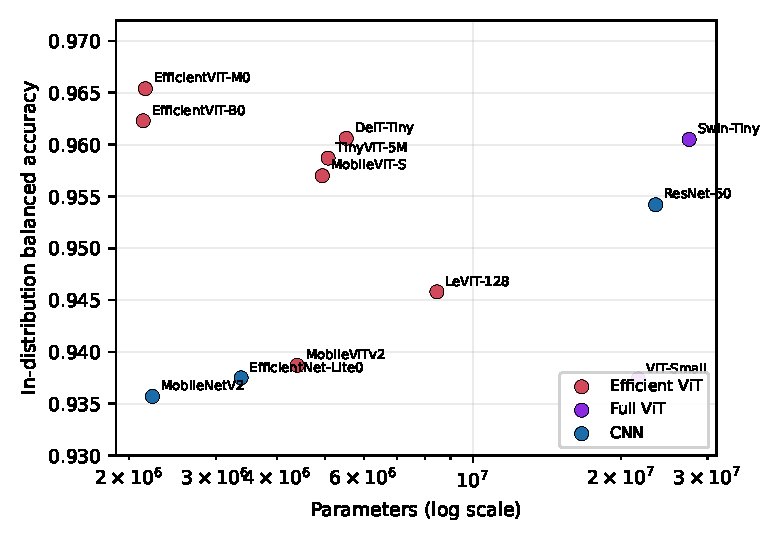
\includegraphics[width=0.82\textwidth]{figs/p1_fig1_params_vs_accuracy.pdf}
\caption{Parameters (log scale) vs.\ in-distribution balanced accuracy,
colored by architecture family. The two efficient-ViT models with the
fewest parameters (EfficientViT-M0/B0) are also the two most accurate.}
\label{fig:params-vs-acc}
\end{figure}

\subsection{Cross-dataset domain shift, escalating from 2 to 12 models}

\textbf{Stage 1 (DeiT-Tiny alone):} in distribution 0.9504 balanced
accuracy, Herlev (zero-shot) 0.7151, Mendeley LBC (zero-shot) 0.5230 -- a
model that looks excellent in distribution degrades to near-chance on the
more severe external dataset, with nothing in a standard pipeline able to
flag this.

\textbf{Stage 2 (adding EfficientViT-M0):} the \emph{better}
in-distribution model (0.9737 vs.\ DeiT-Tiny's 0.9504) is the
\emph{worse} model under both shifts (Herlev 0.6716 vs.\ 0.7151; Mendeley
LBC 0.4731 vs.\ 0.5230 -- the first model in this study to drop below the
0.50 chance floor). Two models this close in architecture family and
parameter count producing this reversal is a direct caution against using
in-distribution accuracy as a proxy for deployment robustness.

\textbf{Stage 3 (adding ResNet-50 and Swin-Tiny):}

\begin{table}[htbp]
\centering
\caption{One model per architecture family under cross-dataset shift.}
\label{tab:rq4-stage3}
\begin{tabular}{lrrr}
\toprule
Model (family) & SIPaKMeD & Herlev & Mendeley LBC \\
\midrule
EfficientViT-M0 (efficient ViT) & \textbf{0.9737} & 0.6716 & \textbf{0.4731} (below chance) \\
Swin-Tiny (full ViT) & 0.9590 & \textbf{0.7282} & 0.5192 \\
DeiT-Tiny (efficient ViT) & 0.9504 & 0.7151 & 0.5230 \\
ResNet-50 (CNN) & 0.9556 & 0.6838 & \textbf{0.6082} \\
\bottomrule
\end{tabular}
\end{table}

Not a clean CNN-vs-transformer split: on Herlev, both transformer models
beat ResNet-50. What holds across both shift datasets is narrower: the
single most parameter-efficient, best-in-distribution model
(EfficientViT-M0) is the worst performer under shift on both external
datasets, and the only one below chance on either.

\textbf{Stage 4 (all 12 models):}

\begin{table}[htbp]
\centering
\caption{Full 12-model cross-dataset shift evaluation, sorted by Mendeley LBC score.}
\label{tab:rq4-full}
\begin{tabular}{lrrr}
\toprule
Model (family, params) & SIPaKMeD & Herlev & Mendeley LBC \\
\midrule
EfficientNet-Lite0 (CNN, 3.38M) & 0.9455 & 0.5970 & \textbf{0.6674} \\
ResNet-50 (CNN, 23.5M) & 0.9556 & 0.6838 & 0.6082 \\
MobileViTv2 (eff.\ ViT, 4.39M) & 0.9638 & \textbf{0.7501} & 0.5418 \\
MobileNetV2 (CNN, 2.23M) & 0.9505 & 0.6919 & 0.5391 \\
DeiT-Tiny (eff.\ ViT, 5.5M) & 0.9504 & 0.7151 & 0.5230 \\
EfficientViT-B0 (eff.\ ViT, 2.14M) & 0.9738 & 0.6818 & 0.5217 \\
Swin-Tiny (full ViT, 27.5M) & 0.9590 & 0.7282 & 0.5192 \\
ViT-Small (full ViT, 21.7M) & 0.9573 & 0.7049 & 0.5084 \\
LeViT-128 (eff.\ ViT, 8.4M) & 0.9526 & 0.5777 & 0.4764 \\
EfficientViT-M0 (eff.\ ViT, 2.16M) & 0.9737 & 0.6716 & 0.4731 \\
TinyViT-5M (eff.\ ViT, 5.1M) & 0.9685 & \textbf{0.7327} & 0.4543 \\
MobileViT-S (eff.\ ViT, 4.94M) & 0.9520 & 0.7104 & \textbf{0.2927} (AUROC 0.215) \\
\bottomrule
\end{tabular}
\end{table}

A near-clean CNN-vs-transformer split emerges on Mendeley LBC, with one
exception: all three CNNs land at 0.539--0.667; eight of nine
transformer-family models land at 0.293--0.523; the ninth (MobileViTv2)
scores 0.5418, above the lowest CNN (0.5391) by 0.003 -- a gap
seed-variance testing (Section~4.4) shows is noise, not a real
difference. This split does not hold on Herlev, where transformer
models occupy both the best (MobileViTv2, TinyViT-5M) and weaker
(LeViT-128) positions.

MobileViT-S is a severe, singular outlier: its Mendeley LBC AUROC (0.215)
is not merely below chance but actively anti-correlated with ground
truth. Its direct successor, MobileViTv2, shows no such problem and is the
single strongest model in the entire registry on Herlev (0.7501) -- the
same architecture-family name spanning a catastrophic failure and a top
performer, ruling out architecture lineage as a predictor of shift
robustness as thoroughly as parameter count and in-distribution accuracy
already have been.

\begin{figure}[htbp]
\centering
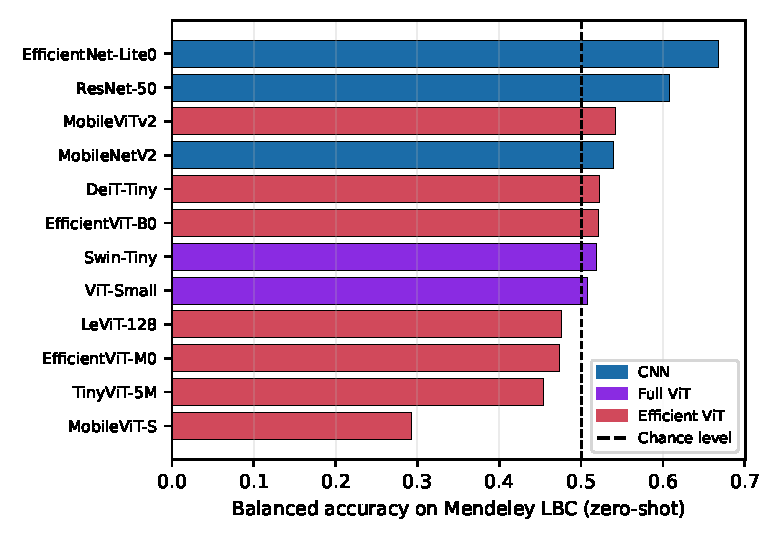
\includegraphics[width=0.82\textwidth]{figs/p1_fig2_mendeley_shift.pdf}
\caption{Balanced accuracy on Mendeley LBC (zero-shot), sorted, colored by
architecture family. All three CNNs cluster above chance; eight of nine
transformer-family models cluster at or below chance, with MobileViT-S
the sole catastrophic outlier.}
\label{fig:mendeley-shift}
\end{figure}

\subsection{A third, independent shift dataset (APCEM)}

\begin{table}[htbp]
\centering
\caption{Full 12-model evaluation on the third external shift dataset (APCEM), sorted by AUROC.}
\label{tab:rq1-apcem}
\begin{tabular}{lrrr}
\toprule
Model (family, params) & SIPaKMeD & APCEM bal.\ acc. & APCEM AUROC \\
\midrule
MobileNetV2 (CNN, 2.23M) & 0.9623 & \textbf{0.6158} & \textbf{0.6528} \\
EfficientNet-Lite0 (CNN, 3.38M) & 0.9309 & 0.5393 & 0.5701 \\
LeViT-128 (eff.\ ViT, 8.4M) & 0.9001 & 0.5263 & 0.5376 \\
Swin-Tiny (full ViT, 27.5M) & 0.9330 & 0.4724 & 0.3082 \\
EfficientViT-B0 (eff.\ ViT, 2.14M) & 0.9638 & 0.4481 & 0.3206 \\
DeiT-Tiny (eff.\ ViT, 5.5M) & 0.9589 & 0.4469 & 0.3799 \\
MobileViTv2 (eff.\ ViT, 4.39M) & 0.9570 & 0.4290 & 0.4120 \\
TinyViT-5M (eff.\ ViT, 5.1M) & 0.9670 & 0.4100 & 0.3681 \\
EfficientViT-M0 (eff.\ ViT, 2.16M) & 0.9621 & 0.3730 & 0.3407 \\
MobileViT-S (eff.\ ViT, 4.94M) & 0.9687 & 0.3621 & 0.3161 \\
ViT-Small (full ViT, 21.7M) & 0.9538 & 0.3444 & 0.2555 \\
ResNet-50 (CNN, 23.5M) & 0.9639 & \textbf{0.3339} & \textbf{0.2929} \\
\bottomrule
\end{tabular}
\end{table}

APCEM is a genuinely independent replication -- different acquisition
pipeline, institution, and label granularity from either Herlev or
Mendeley LBC -- and it does not merely confirm the earlier finding that
in-distribution accuracy fails to predict shift robustness (11 of 12
models land at or below the 0.50 chance floor for balanced accuracy on
APCEM, several with AUROC well below 0.35), it overturns the one pattern
that had looked stable across Stages 3--4: that CNN-family models cluster
above chance while transformer-family models cluster at or below it. Here
the CNN family alone spans the single best-performing model in the entire
registry (MobileNetV2, 0.6158 balanced accuracy, the only model of the 12
to clear chance meaningfully) and one of the single worst (ResNet-50,
AUROC 0.2929, second-lowest of all 12) -- the same family that was the
more robust one, on average, on Mendeley LBC. DeiT-Tiny and
EfficientViT-M0, the two models directly compared since Stage 2, again
replicate their earlier ranking (DeiT-Tiny 0.4469 vs.\ EfficientViT-M0
0.3730), with EfficientViT-M0 again the weaker model under shift despite
again being the stronger in-distribution model on this run (0.9621 vs.\
0.9589) -- the same reversal, now observed on a third, independently
sourced dataset.

\begin{figure}[htbp]
\centering
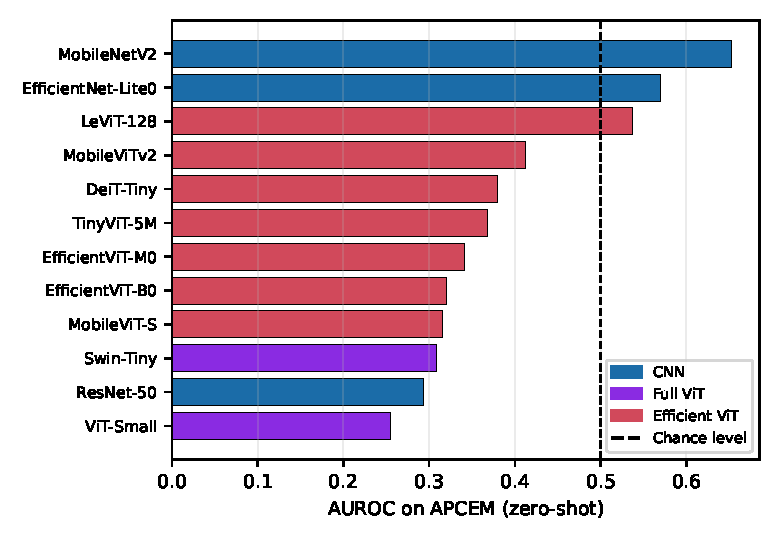
\includegraphics[width=0.82\textwidth]{figs/p1_fig3_apcem_shift.pdf}
\caption{AUROC on APCEM (zero-shot), sorted, colored by architecture
family. Unlike Mendeley LBC, the CNN family spans both the single best
(MobileNetV2) and one of the single worst (ResNet-50) models in the
registry -- no family-level pattern survives this third dataset.}
\label{fig:apcem-shift}
\end{figure}

\subsection{Full-registry seed-variance check: how much of the above is one seed's story?}

Every result above is a single train/val/calibration/test split (seed
13). To test whether the paper's own headline patterns are properties of
the models and datasets, or artifacts of that one seed, we retrained all
12 models at 2 further seeds (17, 29), one training run per model per
seed evaluated zero-shot on all three external datasets from the same
checkpoint, and combined this with the original seed-13 numbers above.

\textbf{The Mendeley LBC ``near-clean CNN-vs-transformer split'' is
itself seed-fragile.} At seed 13, only 1 of 9 transformer-family models
(MobileViTv2, by 0.003) exceeds the weakest CNN. At seed 17, 3 of 9 do,
by margins up to 0.098 (EfficientViT-B0). At seed 29, 4 of 9 do, by
margins up to 0.113. The margins at seeds 17 and 29 are an order of
magnitude past the single close call already flagged as noise at seed 13
-- the ``near-clean split'' description of Mendeley LBC (Section~4.2,
Stage 4) is a property of that specific seed, not a reproducible property
of the dataset or the model families.

\textbf{Herlev's inverse pattern (transformers beating CNNs) is, by
contrast, seed-stable}: 8, 7, and 8 of 9 transformer models exceed the
weakest CNN at seeds 13, 17, and 29 respectively. Not every seed-checked
pattern is fragile.

\textbf{MobileNetV2's APCEM win is seed-stable}: it is the best-performing
model on APCEM at every seed tested (rank 1, 2, and 1 of 12 at seeds 13,
17, 29) -- a genuinely reproducible result, not a single-seed artifact.

\textbf{EfficientViT-M0's specific poster-child reversal is not.} This
paper's running illustration of ``the in-distribution winner is the
shift-robustness loser'' (Sections~1, 4.2) does not reliably occupy
either role across seeds:

\begin{table}[htbp]
\centering
\caption{EfficientViT-M0's in-distribution and shift ranks (of 12) across 3 seeds.}
\label{tab:seedcheck-effvitm0}
\begin{tabular}{lrrr}
\toprule
Seed & In-distribution rank & Herlev shift rank & Mendeley LBC shift rank \\
\midrule
13 & 2 & 10 & 10 \\
17 & 10 & 7 & 7 \\
29 & 1 & 5 & 4 \\
\bottomrule
\end{tabular}
\end{table}

At seed 13, EfficientViT-M0 is (virtually tied for) the in-distribution
winner and one of the worst shift performers on both external datasets --
exactly the reversal illustrated in Section~1. At seed 29, it is the
outright in-distribution winner \emph{and} mid-pack under shift on both
datasets (rank 4--5 of 12) -- no reversal at all. At seed 17 it is not
even the in-distribution winner (rank 10 of 12). This does not weaken the
paper's central claim; if anything it reinforces it. The general claim
this example illustrates -- no static property predicts shift robustness
-- is a further instance of exactly that unreliability, now shown across
seeds of the same model rather than only across different models. What
changes is that this specific model should be read as a seed-13-specific
illustration of the general point, not a reproducible property of
EfficientViT-M0 itself.

\subsection{Uncertainty-quantification comparison}

\begin{table}[htbp]
\centering
\caption{Four uncertainty methods, in distribution and under two external shifts.}
\label{tab:rq2}
\begin{tabular}{lrrrrrrr}
\toprule
Method & \multicolumn{2}{c}{In-dist.} & \multicolumn{2}{c}{Herlev} & \multicolumn{3}{c}{Mendeley LBC} \\
 & ECE & Acc. & RC-AUC & Acc. & RC-AUC & Acc. & Sel.\ acc.@90\% \\
\midrule
Baseline (temp.) & 0.012 & 0.967 & 0.193 & 0.694 & 0.515 & 0.530 & 0.522 \\
MC Dropout & 0.013 & 0.972 & 0.203 & 0.658 & \textbf{0.285} & 0.579 & \textbf{0.583} \\
Evidential & 0.159 & 0.967 & 0.167 & 0.677 & 0.476 & 0.543 & 0.539 \\
Deep ensemble & 0.012 & 0.974 & \textbf{0.147} & \textbf{0.771} & 0.473 & 0.537 & 0.544 \\
\bottomrule
\end{tabular}
\end{table}

\textbf{In distribution, three methods are close; evidential is the
outlier.} Baseline, MC Dropout, and the deep ensemble all calibrate well
(ECE 0.012--0.013) with full-coverage accuracy in the 0.967--0.974 range.
Evidential deep learning's raw belief masses are markedly less calibrated
(ECE 0.159) at matched point accuracy (0.967) -- its probabilities would
need their own post-hoc correction, deliberately not applied here, to
make this comparison's calibration numbers fair to it.

\textbf{Under moderate shift (Herlev), the deep ensemble wins clearly.}
Its risk-coverage AUC (0.147) and full-coverage accuracy (0.771) both beat
the other three methods by a real margin -- member disagreement is doing
genuine, useful work at this shift severity.

\textbf{Under severe shift (Mendeley LBC) -- the condition that matters
most, since it is where this exact backbone is known to fail -- the
ranking inverts.} MC Dropout's entropy is the only signal showing a
substantial, unambiguous improvement over the uncalibrated baseline
(risk-coverage AUC 0.515 to 0.285; full-coverage accuracy 0.530 to 0.579).
Evidential (0.476) and the deep ensemble (0.473) are both only marginally
better than the plain baseline -- essentially within noise of each other
-- despite the ensemble's clear win on the milder shift one row above.
Member disagreement, which correctly flags moderate shift, does not
reliably track the specific failure mode behind the severe collapse.

\subsection{A significance test, and an unexpected non-replication}

To test whether MC Dropout's apparent Mendeley LBC advantage over the deep
ensemble (0.285 vs.\ 0.473) is distinguishable from bootstrap sampling
noise, we ran a paired bootstrap test (2000 resamples) on per-sample
risk-coverage curves. Because only Section~4.5's aggregate metrics, not
its per-sample predictions, had been retained, this required retraining MC
Dropout from scratch -- with the identical seed (13), dropout rate, epoch
budget, and manifest used above -- while the deep ensemble was reloaded
from its five original saved checkpoints. The retrained MC Dropout model
did not reproduce the earlier result: its Mendeley LBC risk-coverage AUC
came out at 0.503, not 0.285, despite every controllable factor being
held fixed. Against this retrained run, the paired bootstrap test found
no statistically significant difference from the deep ensemble (0.503 vs.\
0.474; 95\% CI for the difference $[-0.066, 0.010]$, one-sided
$p=0.929$). This is a stronger and more concerning result than a mere
failure to reach significance: a fixed random seed did not reproduce a
result on this specific severe-shift metric, and the gap between the two
training runs of the identical MC Dropout recipe (0.285 vs.\ 0.503) is
larger than the sampling uncertainty the bootstrap places around either
individual run. To see whether these two runs were themselves a
coincidence, we retrained MC Dropout twice more at genuinely different
seeds (17, 29, otherwise identical recipe): Mendeley LBC risk-coverage AUC
came out at 0.358 and 0.359 -- both landing squarely inside the
0.285--0.503 range the first two runs staked out, rather than clustering
near either endpoint. Four independent training runs of one fixed method
on one fixed backbone now span 0.285 to 0.503, with a spread (0.218) far
larger than the 0.147--0.203 gap that separated any two \emph{different}
methods in Section~4.5's Herlev column. Read together, the four runs mean
the reported severe-shift rank inversion is a property of one specific
trained model, not a property of ``MC Dropout'' as a method on this
backbone -- retraining alone, with no change to data, architecture, or
hyperparameters, was sufficient to erase the reported advantage entirely,
and the method's severe-shift behavior is not concentrated near any
single value at all.

\begin{figure}[htbp]
\centering
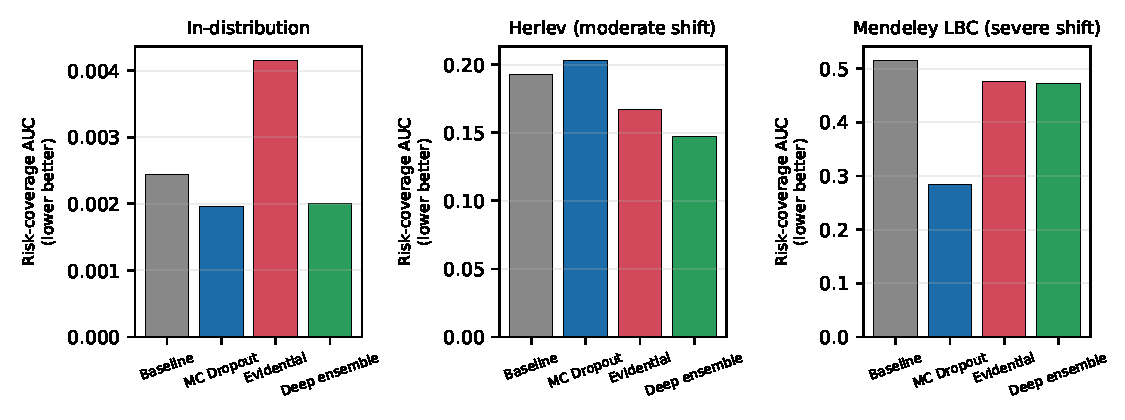
\includegraphics[width=\textwidth]{figs/p2_fig1_risk_coverage.pdf}
\caption{Risk-coverage AUC (lower is better) per method, at three
conditions with independent y-axes (note the $\sim$100$\times$ scale
difference between in-distribution and Mendeley LBC). The best method in
this run changes from deep ensemble (Herlev) to MC Dropout (Mendeley
LBC), though a retraining check found the Mendeley LBC advantage does not
reproduce (see text).}
\label{fig:risk-coverage}
\end{figure}

\textbf{No method reaches a reliable abstention operating point under
severe shift.} Even MC Dropout's best result -- 0.583 selective accuracy
at 90\% coverage on a binary task -- is barely better than chance after
abstaining on the least-confident decile. We report this plainly rather
than treating ``best of four'' as equivalent to ``good enough'': for
deployment purposes, none of these four methods alone would currently
justify an ``abstain and refer'' policy on a shift this severe, in either
run.

\subsection{Explainability comparison}

\begin{table}[htbp]
\centering
\caption{Explainability method comparison, 50 SIPaKMeD test images, all matched to a real nucleus polygon.}
\label{tab:rq3}
\begin{tabular}{lrrr}
\toprule
Method & Deletion AUC$\downarrow$ & Insertion AUC$\uparrow$ & Nucleus conc.$\uparrow$ (1.0 = chance) \\
\midrule
\textbf{Relevancy propagation} & \textbf{0.734} & \textbf{0.970} & \textbf{2.714} \\
Grad-CAM (ViT-adapted) & 0.818 & 0.877 & 1.472 \\
Attention rollout & 0.825 & 0.936 & 1.177 \\
\bottomrule
\end{tabular}
\end{table}

\begin{figure}[htbp]
\centering
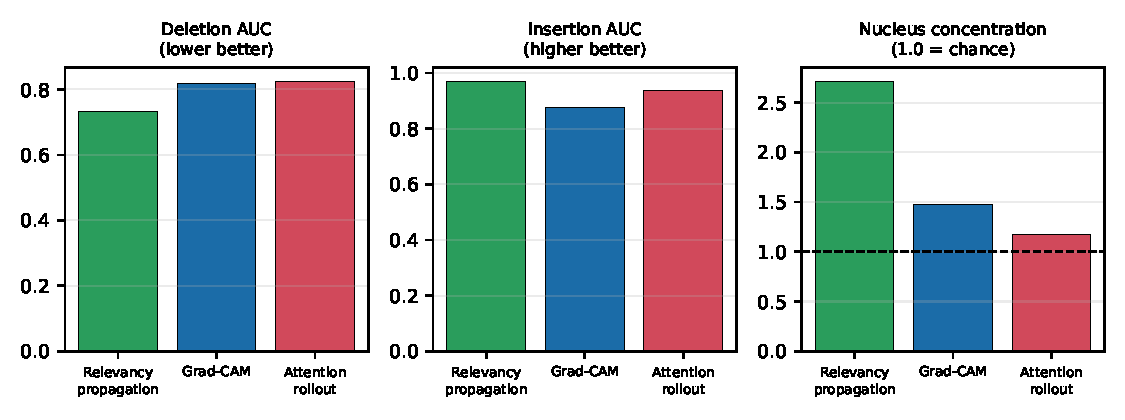
\includegraphics[width=\textwidth]{figs/p3_fig1_explainability_metrics.pdf}
\caption{Deletion AUC, insertion AUC, and nucleus concentration ratio for
the three explainability methods. Relevancy propagation wins on all
three, with the widest margin on nucleus concentration.}
\label{fig:explainability-metrics}
\end{figure}

Relevancy propagation wins every comparison, and by a wide margin on
nucleus concentration specifically (2.71$\times$ chance vs.\ attention
rollout's 1.18$\times$ -- barely above chance). We attribute this to a
mechanistic difference rather than measurement noise: attention rollout
is class-agnostic, an inherent disadvantage on an inherently
class-discriminative faithfulness test, while relevancy propagation is
both class-discriminative \emph{and} integrates the gradient-weighted
signal across all twelve transformer blocks.

\subsection{A second backbone: does the explainability ranking generalize?}

Relevancy propagation's clean, unconditional win is the one result in
this paper that looked, on its face, like it might not need
condition-by-condition re-testing -- but that claim rests on a single
backbone (DeiT-Tiny), so we re-ran the identical comparison on ViT-Small,
a structurally identical \texttt{VisionTransformer} (same
\texttt{global\_pool="token"}, \texttt{num\_prefix\_tokens=1}, 12 blocks
-- verified directly, not assumed) trained fresh with the same recipe and
seed.

\begin{table}[htbp]
\centering
\caption{Explainability ranking on a second backbone (ViT-Small) vs.\ the original (DeiT-Tiny).}
\label{tab:rq3-vit-small}
\begin{tabular}{lrrrrrr}
\toprule
 & \multicolumn{3}{c}{DeiT-Tiny (original)} & \multicolumn{3}{c}{ViT-Small (2nd backbone)} \\
Method & Del.\ AUC$\downarrow$ & Ins.\ AUC$\uparrow$ & Conc.$\uparrow$ & Del.\ AUC$\downarrow$ & Ins.\ AUC$\uparrow$ & Conc.$\uparrow$ \\
\midrule
\textbf{Relevancy prop.} & \textbf{0.734} & \textbf{0.970} & \textbf{2.71} & \textbf{0.816} & \textbf{0.965} & \textbf{4.20} \\
Grad-CAM & 0.818 & 0.877 & 1.47 & 0.888 & 0.895 & 1.35 \\
Attn.\ rollout & 0.825 & 0.936 & 1.18 & 0.888 & 0.927 & 0.97 \\
\bottomrule
\end{tabular}
\end{table}

The ranking replicates exactly: relevancy propagation wins all three
metrics on ViT-Small too, with an even wider nucleus-concentration margin
(4.20$\times$ chance vs.\ its closest competitor's 1.35$\times$) than on
DeiT-Tiny. This is the one property in this paper's tested set that
generalizes cleanly across a backbone change without qualification -- in
contrast to Section~4.9's uncertainty-composition result, which flips
direction depending on shift severity, and Section~4.10's efficiency
claims, which required direct measurement precisely because they did
\emph{not} generalize from architectural reasoning. The generalization
claim is scoped deliberately: both backbones are pure multi-head
self-attention \texttt{VisionTransformer} instances of different widths
and depths, not different architecture families -- whether the ranking
survives a hybrid conv+attention backbone remains untested, since
relevancy propagation is not defined for EfficientViT-M0's architecture
(Section~6, External validity).

\subsection{System-integration: does combining two uncertainty signals help?}

\begin{table}[htbp]
\centering
\caption{Selective-prediction risk-coverage AUC (lower is better): confidence alone vs.\ conformal set size alone vs.\ combined.}
\label{tab:rq5}
\begin{tabular}{lrrr}
\toprule
Condition & Confidence only & Set size only & Combined \\
\midrule
In-distribution & \textbf{0.0050} & 0.0834 & 0.0173 \\
Herlev (moderate shift) & \textbf{0.1190} & 0.3281 & 0.1793 \\
Mendeley LBC (severe shift) & 0.3244 & 0.4395 & \textbf{0.2855} \\
\bottomrule
\end{tabular}
\end{table}

\begin{figure}[htbp]
\centering
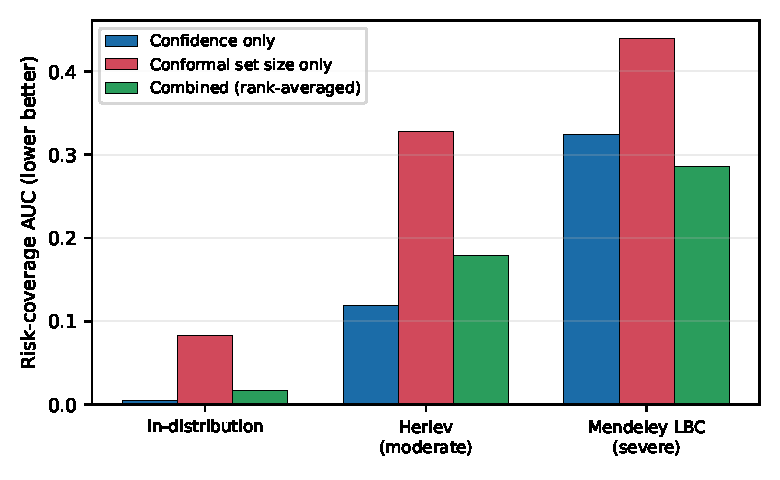
\includegraphics[width=0.85\textwidth]{figs/p3_fig3_combined_selective.pdf}
\caption{Risk-coverage AUC for confidence alone, conformal set size alone,
and the rank-averaged combination, at three conditions. Combining hurts
in-distribution and under moderate shift but helps under severe shift.}
\label{fig:combined-selective}
\end{figure}

Composition is not a uniform win. In distribution and under moderate
shift, confidence alone is already the best individual signal, and
combining it with the noisier discrete conformal-set-size signal dilutes
it. Under severe shift, however, the combined signal is the best of the
three, beating confidence alone. This mirrors the shape of the
uncertainty-method finding in Section~4.5--4.6 (no single choice wins
everywhere), now extended to combinations of signals.

\subsection{Resource efficiency and deployment robustness}

Across the 12-model registry, EfficientNet-Lite0 (3.38M params, 0.77G
FLOPs) has more than 4$\times$ ResNet-50's CPU latency (137.7ms vs.\
32.0ms) despite ResNet-50 having roughly 10$\times$ the FLOPs. Even
EfficientViT-M0, the overall winner on params+FLOPs+accuracy (Section~4.1),
is not the fastest model in wall-clock CPU terms: DeiT-Tiny (15.4ms) and
LeViT-128 (17.5ms) are both faster despite 10--14$\times$ more FLOPs.
EfficientViT-M0, evaluated under synthetic JPEG compression, Gaussian
blur, and brightness/contrast shift, degrades gracefully under all three,
but Gaussian blur is by far the most damaging -- costing 32.8 points of
balanced accuracy at its most severe tested level, roughly double JPEG's
worst case (15.5 points) or brightness/contrast's (18.1 points). A
synthetic OOD sanity check shows mean confidence dropping from 0.985 (real
in-distribution images) to 0.743 (OOD) -- real and meaningful, but far
above the 0.20 chance level for this 5-class task. On CPU, a bare DeiT-Tiny
forward pass has a median latency of 49.6ms; a prediction that also
returns a relevancy-propagation explanation costs 164.1ms -- about
3.3$\times$ the bare-prediction cost.

\begin{figure}[htbp]
\centering
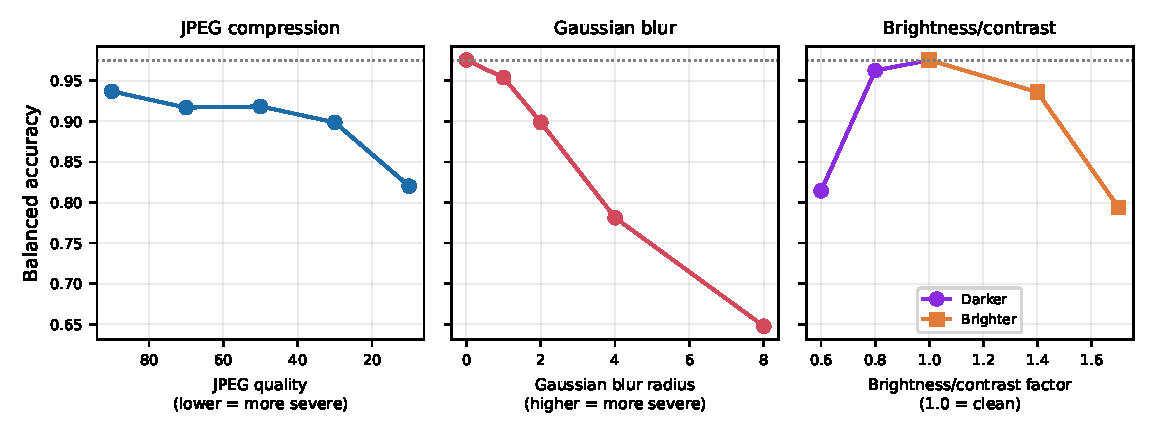
\includegraphics[width=\textwidth]{figs/p3_fig2_degradation_curves.pdf}
\caption{Balanced accuracy vs.\ corruption severity for three synthetic
degradations (EfficientViT-M0, SIPaKMeD test set). The dotted line marks
the clean baseline (0.975). Gaussian blur causes the steepest decline.}
\label{fig:degradation-curves}
\end{figure}

\section{Discussion}

Seven findings, read together, argue against a single verification
strategy applied uniformly to a trustworthy medical AI pipeline. On
\textbf{efficiency and shift robustness} (Sections~4.1--4.4): ``smaller is
worse'' is directly falsified in distribution; ``the in-distribution
winner is the safe choice'' is directly falsified under shift, and
replicates this reversal on a third, independently sourced dataset;
``architecture family/lineage predicts robustness'' is falsified by
MobileViT-S and MobileViTv2 sharing a name and lineage while producing a
catastrophic failure and a top performance on the same evaluation; and,
visible only once a third shift dataset and a seed-variance check are
both added, even a robustness pattern that survives two independent shift
datasets, and even the specific model used to illustrate the paper's own
central claim, are not guaranteed to survive a third shift dataset or a
different random seed respectively. A reader who stopped at two shift
datasets and one seed would have concluded ``CNNs are the robust family''
and ``EfficientViT-M0 is reliably the in-distribution-winner-becomes-
shift-loser example''; both conclusions are one seed or one dataset away
from being overturned.

On \textbf{uncertainty quantification} (Sections~4.5--4.6): a reader who
evaluated the four methods only in distribution, or only under the milder
of the two shifts tested, would conclude the deep ensemble is the best
choice and MC Dropout is mediocre -- the opposite of what the severe-shift
evaluation shows in our original run. The significance test and repeated
retraining add a second, sharper layer to this same warning: it was not
enough for MC Dropout's severe-shift advantage to fail a bootstrap
significance test against the ensemble -- retraining the exact same
method with the exact same seed produced a qualitatively different result
(0.285 becoming 0.503), large enough to flip which method looks better at
all. If a single fixed backbone choice cannot be assumed safe across
shift conditions (Sections~4.1--4.4), and a single fixed uncertainty-method
choice cannot be assumed safe across shift conditions either, this result
adds a third, more uncomfortable layer: a single uncertainty-method
\emph{evaluation run} cannot be assumed to represent that method's
behavior on a severe shift, even holding the seed fixed.

On \textbf{explainability, composition, and measured cost}
(Sections~4.7--4.10): explainability method choice produced the cleanest,
most unambiguous result in the entire paper -- relevancy propagation wins
every metric, with no condition-dependent flip, and the ranking
replicates exactly on a second backbone -- while uncertainty method
choice, uncertainty-signal composition, and architecture-family robustness
patterns all produced conditional, no-single-winner, or seed-dependent
results. This asymmetry suggests that for this task and backbone family,
picking the right explainability method is a more reliably beneficial,
one-time engineering decision than picking (or combining) the right
uncertainty-quantification method or trusting a single seed's robustness
ranking, where the honest answer is ``it depends, and needs re-testing.''
Every efficiency and robustness claim, meanwhile, required direct
measurement to be trusted: FLOP count did not predict CPU latency, and
OOD confidence dropped only partially, not to the clean near-chance level
a reader might assume from an ``OOD detection'' framing.

Together, these seven findings do not all fail to compose the same way --
that is the point. Some properties (explainability method choice) are
robust once tested with reasonable care. Some (uncertainty method choice,
signal composition) are conditional on an operating regime that must be
identified before trusting any single-condition evaluation. Some
(architecture-family robustness patterns, and even which specific model
best illustrates a general claim) are not safely generalized beyond the
exact seed and dataset used to establish them, and require deliberate,
repeated re-testing to distinguish a real pattern from a one-run
artifact. A system designer who validates one of these properties once
and assumes the others behave the same way is making an assumption this
data does not support, at three different levels: across models, across
shift datasets, and across random seeds of the identical model and
recipe.

\section{Threats to Validity}

\textbf{Internal validity.} Each headline model in Sections~4.1--4.3 was
trained once (seed 13); Section~4.4 measured seed-to-seed variance
directly across all 12 models at 2 further seeds (17, 29) rather than
leaving it as a caveat, and found some specific single-model,
single-dataset claims (the Mendeley LBC CNN-vs-transformer split,
EfficientViT-M0 as the in-distribution-winner-becomes-shift-loser
example) are seed-fragile, while others (Herlev's inverse pattern,
MobileNetV2's APCEM win) are seed-stable -- Section~4.4 gives the full
breakdown. No trained-weight checkpoints persist across sessions, so
results could not be re-verified from the original weights without full
retraining; the reported numbers are the direct, unedited output of the
released training and evaluation code, which mitigates but does not
eliminate this threat. For the uncertainty-quantification comparison
(Sections~4.5--4.6), this threat is no longer hypothetical: we tested it
directly by retraining MC Dropout three more times (seed 13 again, then
genuinely different seeds 17 and 29), all under the identical dropout
rate, epoch budget, and manifest used for Table~5. The four Mendeley LBC
risk-coverage AUC values -- 0.285, 0.503, 0.358, 0.359 -- span 0.218, with
the two seed-17/29 runs landing in between the two nominally-seed-13 runs
rather than clustering near either. This swing erases the reported
severe-shift advantage entirely and makes at least one retrained run
statistically indistinguishable from the deep ensemble (paired bootstrap
95\% CI for the difference $[-0.066, 0.010]$, one-sided $p=0.929$;
Section~4.6). The deep ensemble's 5 members use one fixed set of seeds,
reused unchanged for this significance test; seed-to-seed ensemble
variance was not separately measured. For the explainability comparison
(Sections~4.7--4.8), the 50-image evaluation sample is one fixed
stratified sample (10 per class); a different sample could shift the
exact deletion/insertion/nucleus-concentration numbers, though the margin
by which relevancy propagation wins on all three metrics, on both
backbones, is large enough that a resampling-driven reversal of the
ranking is unlikely. The OOD sanity check's 25-image sample (Section~4.10)
is smaller still, and its qualitative conclusion (confidence drops but not
to chance) should be treated as suggestive rather than a precise estimate
for this reason. CPU latency figures (Section~4.10) were measured on one
shared consumer laptop rather than isolated benchmark hardware; a
$\sim$30\% run-to-run swing was observed for the same model, so the exact
3.3$\times$ explanation-cost multiplier should be read as approximate,
not a precise constant, though relative ordering across models was
stable.

\textbf{External validity.} All four datasets are drawn from a small
number of source institutions (SIPaKMeD, Herlev, Mendeley LBC, and APCEM
together represent four geographic/clinical sources), and generalization
to other scanners, staining protocols, or populations beyond these four is
not established. The three shift conditions tested (Herlev, Mendeley LBC,
APCEM) are real cross-institution shifts, not a systematic sweep across
shift types (e.g., scanner resolution, stain intensity, patient
demographics varied independently), so the finding that no static model
property predicts shift robustness is demonstrated for these three shifts
specifically, not proven for shift in general. The APCEM result itself is
direct evidence for why this caveat matters in practice, not just in
principle: the CNN-family robustness pattern that held across the first
two shift datasets did not survive the third, so a reader should not
assume the specific findings reported here (e.g., which individual model
is most robust) transfer to a fourth, untested shift condition either --
only the higher-level conclusion, that no static property reliably
predicts shift robustness, is expected to generalize. The
uncertainty-quantification comparison (Sections~4.5--4.6) uses a single
backbone (EfficientViT-M0) and two shift conditions; whether the same rank
inversion (ensemble best under moderate shift, MC Dropout best under
severe shift) would recur with a different backbone, a third shift
condition, or a continuous rather than two-point severity scale is
untested and is the most direct follow-up this result motivates. The
explainability ranking (Sections~4.7--4.8) was re-tested on a second
backbone, ViT-Small, and replicated exactly, but both DeiT-Tiny and
ViT-Small are standard multi-head self-attention transformers of the same
architectural family, chosen specifically because relevancy propagation
is defined for them and not for EfficientViT-M0's hybrid design; this
closes the single-backbone gap only within that family. The
selective-prediction composition result and the degradation/OOD findings
(Sections~4.9--4.10) were not re-tested on ViT-Small and still use
DeiT-Tiny alone. Whether any of the explainability, composition, or
degradation/OOD results transfer to a hybrid conv+attention backbone, or
to a different medical imaging task entirely, remains untested.

\textbf{Construct validity.} Balanced accuracy, macro F1, and AUROC
(Sections~4.1--4.4) are standard, well-understood metrics for imbalanced
multi-class classification, reducing the risk that the efficiency or
robustness claims are artifacts of an unusual metric choice. Measured
CPU/GPU latency is a single-run, single-batch-size figure per model and
is not the focus of the paper's central efficiency/robustness claims, so
its precision is secondary to those findings. Risk-coverage AUC and
selective accuracy at fixed coverage (Sections~4.5--4.6) are standard
selective-prediction metrics with clear operational meaning, reducing the
risk that the rank inversion is an artifact of an unusual metric choice.
Evidential deep learning's calibration numbers are reported without the
post-hoc correction its raw outputs would need for a fully fair comparison
to the other three methods' already-calibrated numbers -- a known
asymmetry in how the four methods are scored, stated explicitly rather
than smoothed over. Deletion/insertion AUC and nucleus concentration
ratio (Sections~4.7--4.8) are both well-established or directly
interpretable metrics, reducing the risk that the explainability ranking
is an artifact of an unusual scoring choice; using SIPaKMeD's own
expert-marked nucleus polygons as ground truth, rather than a
segmentation model's derived output, specifically avoids compounding this
evaluation with a second model's own errors. No clinical or expert-review
validation of explanation localization fidelity was performed anywhere in
this paper -- agreement with a nucleus boundary is not equivalent to a
cytotechnologist judging an explanation clinically meaningful, a
distinction stated explicitly rather than implied away.

\section{Limitations}

Three external shift datasets, all drawn from a small number of source
institutions; the shift conditions tested here are real but not
exhaustive of the shift a deployed system might encounter, and the
architecture-family pattern found stable across the first two shift
datasets did not survive the third, so any single-dataset robustness
ranking reported here should be read as specific to that dataset rather
than as a general robustness ordering. Each Section~4.1--4.3 headline
result is a single train/val/calibration/test split (seed 13); results are
not averaged over multiple seeds by default, though seed-to-seed variance
was measured directly (Section~4.4, Section~6 Internal validity) across
all 12 models at 2 further seeds rather than left unmeasured, and that
check found some single-model and single-dataset claims are seed-specific
rather than general, so individual rows and close-ranked comparisons in
these tables should be read with that caution; the paper's higher-level
conclusions do not rest on any single seed-fragile comparison. No
trained-weight checkpoints persist; reproducing any single row of these
tables means retraining from scratch. The uncertainty-quantification
comparison (Sections~4.5--4.6) uses a single backbone (EfficientViT-M0);
whether the reported inversion (ensemble best under moderate shift, MC
Dropout best under severe shift) holds for other architectures is
untested, and its own severe-shift ranking was directly shown not to
reproduce under retraining (the paper's own central caution here).
``Moderate'' and ``severe'' shift are descriptive labels based on the
accuracy drop observed, not independently validated shift-magnitude
measurements. Evidential deep learning's calibration numbers are reported
without the post-hoc correction its raw outputs would need for a fully
fair comparison. Deep ensemble results depend on the specific 5 seeds
used; seed-to-seed ensemble variance was not separately measured. The
explainability and system-integration results (Sections~4.7--4.10) use
DeiT-Tiny, not the efficiency benchmark's overall winner, EfficientViT-M0,
since relevancy propagation is not defined for the latter; the
explainability ranking specifically was confirmed on one additional
same-family backbone (ViT-Small), but whether any of these results
transfer to a hybrid conv+attention backbone remains untested. CPU latency
measured on one shared consumer laptop, not dedicated hardware; a
$\sim$30\% run-to-run swing was observed for the same model, though
relative ordering across models was stable. The OOD sanity check uses a
small, synthetic sample (25 images) rather than a natural out-of-domain
dataset. No clinical or expert-review validation of explanation
localization fidelity was performed anywhere in this paper.

\section{Conclusion}

Testing five independently-varying properties of one trustworthy cervical
cytology screening pipeline, side by side rather than one at a time, does
not produce one story -- it produces three. Some properties resolve
cleanly and hold up under scrutiny: relevancy propagation is unambiguously
the most faithful of three explainability methods tested, on both
behavioral faithfulness and real expert-annotated localization ground
truth, and this ranking replicates exactly on a second, independently-
trained backbone. Some properties resolve conditionally, flipping
direction with the operating regime: composing two uncertainty signals
for selective prediction helps only where the better individual signal
was already failing, and the uncertainty-quantification method that wins
under moderate distribution shift is not the method that wins under
severe shift. And some properties that look stable turn out to be
artifacts of a single seed, dataset, or trained instance once tested
again under identical conditions: a CNN-family robustness pattern that
survived two external shift datasets collapsed on a third; this paper's
own headline illustration of an in-distribution winner becoming a
shift-robustness loser does not reliably reproduce across random seeds of
the identical model; and an uncertainty method's reported advantage under
severe shift vanished on retraining with the identical seed and recipe,
with four independent runs spanning a wider gap than separates any two
different methods. Twelve models across three architecture families also
show, contrary to the usual efficiency-accuracy trade-off framing, that
parameter-efficient vision transformers cost nothing here -- the smallest
models in the registry are also the most accurate in distribution -- and
resource-efficiency claims for lightweight architectures resolve only
under direct measurement, in both directions: FLOP-efficient does not mean
latency-efficient, and ``confidence drops on OOD input'' does not mean
``confidence reaches a safe abstention level.'' No single verification
strategy -- pick the best method once, assume a pattern generalizes across
datasets, trust that a fixed seed represents a method's behavior, or trust
an architectural efficiency claim without measuring it -- would have
correctly characterized all five properties of this one pipeline tested
here; each required its own test, repeated where a single run could not
answer the question, on its own terms.

\begin{thebibliography}{99}

\bibitem{plissiti2018sipakmed}
Plissiti, M.E., Dimitrakopoulos, P., Sfikas, G., Nikou, C., Krikoni, O.,
Charchanti, A.: SIPAKMED: A new dataset for feature and image based
classification of normal and pathological cervical cells in Pap smear
images. In: 2018 IEEE International Conference on Image Processing
(ICIP), pp.\ 3144--3148 (2018)

\bibitem{he2016resnet}
He, K., Zhang, X., Ren, S., Sun, J.: Deep residual learning for image
recognition. In: CVPR (2016)

\bibitem{sandler2018mobilenetv2}
Sandler, M., Howard, A., Zhu, M., Zhmoginov, A., Chen, L.C.: MobileNetV2:
Inverted residuals and linear bottlenecks. In: CVPR (2018)

\bibitem{tan2019efficientnet}
Tan, M., Le, Q.: EfficientNet: Rethinking model scaling for convolutional
neural networks. In: ICML (2019)

\bibitem{dosovitskiy2021vit}
Dosovitskiy, A., et al.: An image is worth 16x16 words: Transformers for
image recognition at scale. In: ICLR (2021)

\bibitem{liu2021swin}
Liu, Z., Lin, Y., Cao, Y., Hu, H., Wei, Y., Zhang, Z., Lin, S., Guo, B.:
Swin Transformer: Hierarchical vision transformer using shifted windows.
In: ICCV (2021)

\bibitem{touvron2021deit}
Touvron, H., Cord, M., Douze, M., Massa, F., Sablayrolles, A., J\'egou,
H.: Training data-efficient image transformers \& distillation through
attention. In: ICML (2021)

\bibitem{graham2021levit}
Graham, B., El-Nouby, A., Touvron, H., Stock, P., Joulin, A., J\'egou, H.,
Douze, M.: LeViT: a vision transformer in ConvNet's clothing for faster
inference. In: ICCV (2021)

\bibitem{wu2022tinyvit}
Wu, K., et al.: TinyViT: Fast pretraining distillation for small vision
transformers. In: ECCV (2022)

\bibitem{mehta2022mobilevit}
Mehta, S., Rastegari, M.: MobileViT: Light-weight, general-purpose, and
mobile-friendly vision transformer. In: ICLR (2022)

\bibitem{mehta2022mobilevitv2}
Mehta, S., Rastegari, M.: Separable self-attention for mobile vision
transformers. arXiv preprint (2022)

\bibitem{cai2023efficientvit}
Cai, H., Li, J., Hu, M., Gan, C., Han, S.: EfficientViT: Multi-scale
linear attention for high-resolution dense prediction. In: ICCV (2023)

\bibitem{liu2023efficientvit}
Liu, X., Peng, H., Zheng, N., Yang, Y., Hu, H., Yuan, Y.: EfficientViT:
Memory efficient vision transformer with cascaded group attention. In:
CVPR (2023)

\bibitem{jantzen2005herlev}
Jantzen, J., Norup, J., Dounias, G., Bjerregaard, B.: Pap-smear benchmark
data for pattern classification. In: Proceedings of Nature Inspired Smart
Information Systems (NiSIS), pp.\ 1--9 (2005)

\bibitem{hussain2020mendeley}
Hussain, E., Mahanta, L.B., Borah, H., Das, C.R.: Liquid based-cytology
Pap smear dataset for automated multi-class diagnosis of pre-cancerous
and cervical cancer lesions. Data in Brief 30, 105589 (2020)

\bibitem{aswini2026apcem}
Aswini, H.: APCEM-Enhanced Cervical Cytology Image Dataset (Version 2)
[Data set]. Mendeley Data (2026). \url{https://doi.org/10.17632/snzb5g6ddy.2}

\bibitem{guo2017calibration}
Guo, C., Pleiss, G., Sun, Y., Weinberger, K.Q.: On calibration of modern
neural networks. In: ICML (2017)

\bibitem{gal2016dropout}
Gal, Y., Ghahramani, Z.: Dropout as a Bayesian approximation:
Representing model uncertainty in deep learning. In: ICML (2016)

\bibitem{lakshminarayanan2017ensembles}
Lakshminarayanan, B., Pritzel, A., Blundell, C.: Simple and scalable
predictive uncertainty estimation using deep ensembles. In: NeurIPS (2017)

\bibitem{sensoy2018evidential}
Sensoy, M., Kaplan, L., Kandemir, M.: Evidential deep learning to
quantify classification uncertainty. In: NeurIPS (2018)

\bibitem{chefer2021transformer}
Chefer, H., Gur, S., Wolf, L.: Transformer interpretability beyond
attention visualization. In: CVPR (2021)

\bibitem{abnar2020quantifying}
Abnar, S., Zuidema, W.: Quantifying attention flow in transformers. In:
ACL (2020)

\bibitem{selvaraju2017gradcam}
Selvaraju, R.R., Cogswell, M., Das, A., Vedantam, R., Parikh, D., Batra,
D.: Grad-CAM: Visual explanations from deep networks via gradient-based
localization. In: ICCV (2017)

\bibitem{petsiuk2018rise}
Petsiuk, V., Das, A., Saenko, K.: RISE: Randomized input sampling for
explanation of black-box models. In: BMVC (2018)

\bibitem{mohiuddin2025}
Mohiuddin, A.B., Rahman, M.M., et al.: Accelerated and accurate cervical
cancer diagnosis using a novel stacking ensemble method with explainable
AI. In: International Conference on Quantum Photonics, Artificial
Intelligence (2025)

\bibitem{rahman2026maizeformerx}
Rahman, M.M., et al.: MaizeFormerX: a lightweight vision transformer with
cross-scale attention for explainable maize leaf disease diagnosis.
Scientific Reports (2026)

\bibitem{gony2026retinal}
Gony, M.N., Shuvra, S.M.K., Poudel, R., Dhakal, K., Rahman, M.M., et al.:
Dual-view semi-supervised retinal disease recognition via chromatic
structural decomposition and cross-view contrastive learning. In:
International Conference on Power, Electronics, Communications (2026)

\bibitem{ahmed2026postsurgical}
Ahmed, M., Ahmed, F., Mow, S.M., Taha, P.A., Barua, S., Rahman, M.M., et
al.: An explainable multimodal AI framework with reinforcement learning
for post-surgical clinical decision support. medRxiv (2026)

\end{thebibliography}
\end{document}
